\section{Gatos Gemelos}

\begin{figure}[htbp]
\begin{center}
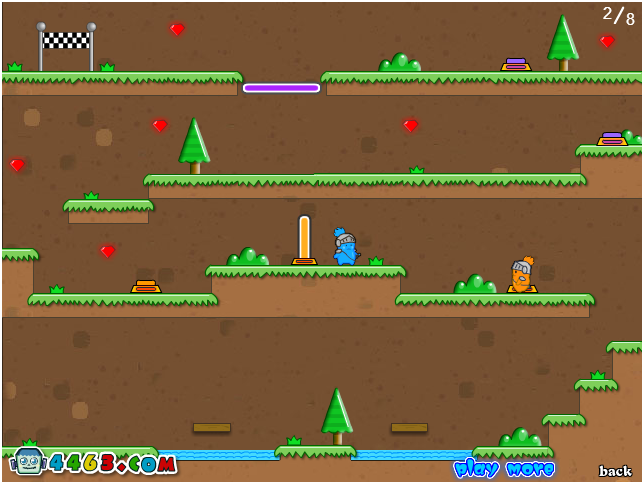
\includegraphics[width=.60\textwidth]{./imagenes/gatos.png}
\caption{Gatos Gemelos}
\label{Gatos Gemelos}
\end{center}
\end{figure}
Gatos Gemelos \footnote{\url{http://ar.yayoye.com/twin-cat-online-game/22643/}} es un Juego en el que se deben mover a los personajes por la pantalla, como su nombre mismo lo dice son unos gatos gemelos, con los que iremos tratando de recoger diamantes y de lograr que interactúen entre ellos para superar los obstáculos.

\subsubsection{¿Por qué es uno de mis juegos favoritos?}
\begin{itemize}
\item[Tania Sánchez] Las reglas del juego son similares a los anteriores juegos de Zelda con el agregado que ahora cada enemigo fue diseñado con los controles de moviemiento en mente, no basta con agitar de izquierda a derecha el control para poder pasar el juego, y esto ayuda en gran parte a sumergirte en el juego ya que debes atacar de cierta forma a los enemigos y/o repeler ataques con tu escudo en el momento preciso sino recibes una penalidad. A pesar de esto, el juego no es atractivo para todo el mundo debido a la única opción de controles a los que alegan que no responden con suficiente precisión o a veces ni responden. Para mi, el gran interés del juego, aparte de presentar el origen de la historia del universo de Zelda, es el nuevo estilo de jugarlo y la experiencia de inmersión única que presenta a cualquier fan de la serie (los motion controls de Twilight Princess para Wii no cuentan en mi opinión ya que eran tan solo un test para ver que tan buena sería la acogida para implementarlo como única opción en el siguiente Zelda).
\end{itemize}